


\section{Optimizing Alignment for Matrix Vector Multiplication}
To illustrate how real world applications can be impacted by aliasing, we look at low level numerical applications.
In this section we show that even highly optimized numerical libraries suffer performance degradation from aliasing.
Basic Linear Algebra Subroutines (BLAS), is the de facto standard API for high performance linear algebra routines.
The functionality is divided into three categories: 

\begin{description}
  \item{Level~1} Scalar and vector operations, such as dot product and vector addition.
  \item{Level~2} Matrix-vector operations, such as gemv for general matrix-vector multiplication.
  \item{Level~3} Matrix-matrix operations, including the widely applied gemm routine for general matrix-matrix multiplication. 
\end{description}

Functions operating on vectors, from BLAS Level 1 or 2, intuitively appears the most likely to have potential for aliasing.
Many highly optimized implementations of BLAS exists, ATLAS being a widely used and open source alternative. One of the key features of ATLAS is that it uses automatic tuning to optimize for cache efficiency [Whaley:2000:ATLAS]. 

\pgfplotstableread{bin/libblas.dat}{\libblastable}
\pgfplotstableread{bin/libatlas.dat}{\libatlastable}
\pgfplotstableread{bin/libopenblas.dat}{\libopenblastable}
\begin{figure}[t]
  \centering
  \begin{tikzpicture}
    \begin{axis}[
        title=libblas,
        font=\footnotesize,
        xlabel=Address offset of vector $y$,
        %ylabel=Event count,
        cycle list name=black white,
        width=\textwidth/2.5, % Make it fit to text width side by side
        legend style={anchor=north east}
      ]
      \addplot table[x expr = \thisrowno{0}, y = cycles:u] \libblastable ;
      \addplot table[x expr = \thisrowno{0}, y = r0107:u ] \libblastable ;
      %\addlegendentry{Cycles} ;
      %\addlegendentry{Alias} ;
    \end{axis}
  \end{tikzpicture}
  \begin{tikzpicture}
    \begin{axis}[
        title=libatlas,
        font=\footnotesize,
        xlabel=Address offset of vector $y$,
        %ylabel=Event count,
        cycle list name=black white,
        width=\textwidth/2.5,
        % skip coords between index={20}{32}
      ]
      \addplot table[x expr = \thisrowno{0}, y = cycles:u] \libatlastable ;
      \addplot table[x expr = \thisrowno{0}, y = r0107:u ] \libatlastable ;
      %\addlegendentry{Cycles} ;
      %\addlegendentry{Alias} ;
    \end{axis}
  \end{tikzpicture}
  \begin{tikzpicture}
    \begin{axis}[
        title=libopenblas,
        font=\footnotesize,
        xlabel=Address offset of vector $y$,
        %ylabel=Event count,
        cycle list name=black white,
        width=\textwidth/2.5,
        % skip coords between index={20}{32}
      ]
      \addplot table[x expr = \thisrowno{0}, y = cycles:u] \libopenblastable ;
      \addplot table[x expr = \thisrowno{0}, y = r0107:u ] \libopenblastable ;
      %\addlegendentry{Cycles} ;
      %\addlegendentry{Alias} ;
    \end{axis}
  \end{tikzpicture}
  \label{fig:conv-default}
  \caption{Wat is dis}
\end{figure}





\section{Optimizing Alignment in BLAS}

To illustrate how real world applications can be impacted by aliasing, we look at low level numerical applications.
In this section we show that even highly optimized numerical libraries suffer performance degradation from aliasing.
Basic Linear Algebra Subroutines (BLAS), is the de facto standard API for high performance linear algebra routines.
The functionality is divided into three categories: 

\begin{description}
  \item{Level~1} Scalar and vector operations, such as dot product and vector addition.
  \item{Level~2} Matrix-vector operations, such as gemv for general matrix-vector multiplication.
  \item{Level~3} Matrix-matrix operations, including the widely applied gemm routine for general matrix-matrix multiplication. 
\end{description}

Functions operating on vectors, from BLAS Level 1 or 2, intuitively appears the most likely to have potential for aliasing.
Many highly optimized implementations of BLAS exists, ATLAS being a widely used and open source alternative. One of the key features of ATLAS is that it uses automatic tuning to optimize for cache efficiency [Whaley:2000:ATLAS]. 

We use the currently latest stable version 3.10.1 of ATLAS, built as a shared library from source.
The automatic tuning happens during the build process; A series of test programs are run to determine cache edges and other properties of the hardware, which in turn affects the resulting binary. 

Carefully monitoring cache metrics is particularly important in this case study, as BLAS performance heavily relies on cache efficiency.
Relevant performance statistics for cache hit ratios was considered to rule out cache as the cause of any bias effects.
In addition, we disable hardware prefetching in BIOS to further minimize cache impacts. 
Note however that the same conclusions can be drawn independently of these measures.

\subsection{Aliasing in cblas\_daxpy}
Found aliasing here as well. Two spikes, not sure why. Might want to test other BLAS libraries. Include or leave out? Too much handwaving and too little analysis maybe. Depends on the target paper length as well?



\subsection{Matrix vector multiplication}

Consider matrix-vector multiplication of the form $\boldsymbol{y} = A\boldsymbol{x} + \boldsymbol{b}$.
Let A be of size $M \times N$, where M is the number of rows. 

$
\left[\begin{array}{ccccc}
a_{0,0} & a_{0,1} &  &  & a_{0,N}\\
a_{1,0}\\
 &  &  & \ddots\\
a_{M,0} &  &  &  & a_{M,N}
\end{array}\right]\left[\begin{array}{c}
x_{0}\\
x_{1}\\
\vdots\\
\\
x_{N}
\end{array}\right]=\left[\begin{array}{c}
y_{0}\\
y_{1}\\
\vdots\\
y_{M}
\end{array}\right]
$

General matrix vector multiplication is implemented by the level 2 gemv routine, computing $\boldsymbol{y} = \alpha\text{op}\left(A\right)\boldsymbol{x} + \beta\boldsymbol{y}$
Here, $\alpha$ and $\beta$ are constants, and $\text{op}\left(A\right)$ is an optional transpose or complex conjugate of the matrix. 
We set $\alpha = 1$, $\beta = 0$ and $\text{op} \left(A\right) = A$ to reduce the formula to $\boldsymbol{y}=A\boldsymbol{x}$.
[There are three memory buffers involved, and one might suspect that implementations are succeptible to aliasing between of $\boldsymbol{A}$, $\boldsymbol{x}$ or $\boldsymbol{y}$.]
For the following discussion we look at a particular configuration where $A$ is of size $64\times64$.

In order to accurately measure any effects of aliasing, we need to isolate the actual function call from heap allocation and initialization code.
This is done by running the program twice for each memory configuration, one where cblas\_dgemv is executed $K = 101$ times in a tight loop.
An approximation of the cost for a single function invocation can be expressed as 
$$
t_{\text{estimate}}=\frac{t_{K=101}-t_{K=1}}{100}
$$
where t represents some metric, such as the number of cycles.
Subtracting the $K = 1$ run removes the constant overhead from the $K = 101$ run, and dividing by $100$ averages the values from the remaining iterations.
Other iteration counts could have been used as well.

Figure \ref{fig:heatmap} shows estimated number of alias events for every relevant memory configuration possible for cblas\_dgemv with matrix size 64 $\times$ 64. 
While matrix A is kept fixed at address suffix 0x000, every reasonable variation of (\&x, \&y) is measured.
Each increment represents an address offset of 16 bytes, which is the same granularity one would get from the default heap allocator.
In a 4K address space, there are thus $4096/16 = 256$ possible address suffixes for $\boldsymbol{x}$ and $\boldsymbol{y}$ independently, resulting in a grid of $256^2$ values.

\begin{figure}[h]
  \caption{Estimated aliasing cost of invoking cblas\_dgemv with a matrix size $64 \times 64$ for different memory layouts. Axis show address offsets times 0x10 for vectors $\boldsymbol{x}$ and $\boldsymbol{y}$. Matrix $A$ has fixed to address suffix 0x000.}
  \label{fig:heatmap}
  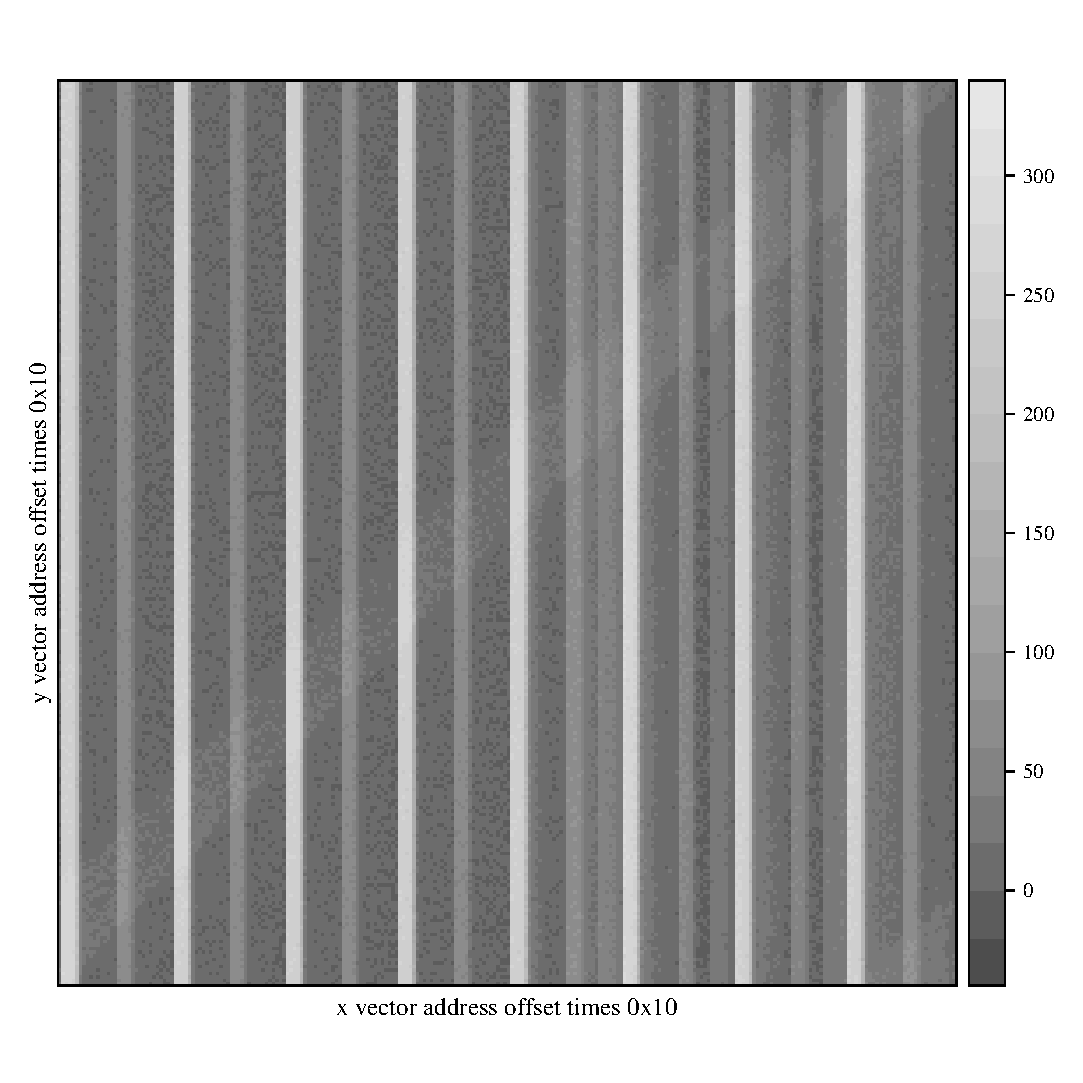
\includegraphics[width=\columnwidth]{resources/heatmap.eps}
\end{figure}

It appears that aliasing is mostly dependent on the location of $\boldsymbol{y}$, in this case with 8 distinct worst case regions.
This is consistent with false dependencies between $\boldsymbol{y}$ and specific rows in A. 
The first bad region is where $\&y ~= 0$, matching the first row of A. 



\begin{table*}[t]
  \caption{Estimated cost of invoking cblas\_dgemv with a matrix size $8192 \times 8192$}
  \label{tab:atlas8k}
  \small
  \centering
  \begin{tabular}{l r r r}
    \toprule
      & (0x010, 0x010, 0x020) & (0x010, 0x010, 0x0b0) & (0x010, 0x140, 0x150) \\
    \midrule
    \perfctr{cpu_clk_unhalted.thread_p} & 162,926,895 & 152,151,263 & 144,583,160 \\
    \perfctr{ld_blocs_partial.address_alias} & \textbf{68,408,790} & \textbf{5,154,981} & \textbf{2,919} \\

    \perfctr{mem_uops_retired.all.loads} & 100,701,777 & 100,702,138 & 100,701,752 \\
    \perfctr{mem_load_uops_retired.hit_lfb} & 31,628,539 & 32,495,287 & 29,853,850 \\
    \perfctr{mem_load_uops_retired.l1_hit} & 68,309,447 & 65,625,881 & 69,387,368 \\
    \perfctr{mem_load_uops_retired.l2_hit} & 711,973 & 1,540,956 & 864,720 \\
    \perfctr{mem_load_uops_retired.l3_hit} & 154,345 & 651,985 & 363,331 \\
    \perfctr{mem_load_uops_retired.l3_miss} & 106,313 & 350,449 & 295,235 \\
    \perfctr{mem_load_uops_retired.all_stores} & 33,562,692 & 33,562,692 & 33,562,692 \\

    \perfctr{load_hit_pre.hw_pf} & 42,914,191 & 47,315,935 & 59,211,320 \\
    \bottomrule
  \end{tabular}
\end{table*}

Notes: 
 - More BR\_INST.COND.TAKEN taken in case (a), but number of retired instructions are the same. Suggests replays of instructions.
 - Inverse HW prefetch numbers from masters

\paragraph{Prefetching}
Measurements repeated with prefetching disabled, giving similar results. 

Estimated performance counter statistics for each of the three heap address configurations are shown in Table [?tab:gemv-estimate].
In addition to cycle count and alias events, a number of relevant metrics related to cache activity are also included.
Notice that almost all load micro-ops are served by either the line fill buffer or L1 cache in all cases.
Only a small amount of loads come from L2, and almost none from L3.
The hit rate for L1 actually decreases somewhat (considering LFB as well) with better execution time.
This could be explained by less time for prefetchers to feed the L1 cache with data.
The hardware prefetch counter indicates more hits in cases a and b.
Again, we find that cache efficiency does not explain the performance cliffs we observe. 

Our results show that address aliasing between matrix and vector heap buffers can significantly impact performance of dgemv in ATLAS.
Variations in heap addresses alone can give a speedup of more than 30 \%.


\subsection{Dealing with Aliasing}
For the particular case we investigated, a good heuristic is to align heap segments “far apart” within the 4 KiB area of 12-bit suffixes.
More specifically, it appears that address suffixes of A and $\boldsymbol{y}$ are the most important to separate.

As discussed in section [x], aliasing cases like these can be accounted for in software using padding techniques.
A possible runtime solution to adjust heap addresses can be realized as follows:

\begin{itemize}
  \item Allocate some extra space for one of the vectors when calling malloc, for instance sizeof(double) * (M + 0x100) for $\boldsymbol{y}$.

  \item Check the returned pointers for potential alias, i.e. the difference between \&A and \&y. Offset using pointer arithmetic into the array with extra padding at the end, i.e. y += 0x100. 
\end{itemize}

Another option is to explicitly account for “worst cases” in the implementation of routines that are vulnerable to aliasing.
Addresses can be explicitly checked for potential conflicts in cblas\_dgemv, and if possible branch to code that will not suffer from aliasing. 
